
\begin{dialog}{一首无的奉献\label{abcd}\note{本篇对话中所有真公案皆引自保罗·李普士[Paul Reps]所著《禅肉,禅骨》与吉奥麦·库伯斯的《禅宗公案》。中译文出自无门慧开纂《禅宗无门关》,载于《大藏经》第四十七卷。}}

\begin{quote}
乌龟和阿基里斯刚刚听了一个关于遗传密码起源的讲座,此时他们俩正在阿基里斯家喝茶。
\end{quote}

\begin{dialogue}

\item[阿基里斯]有件不好意思的事我得坦白,龟兄。

\item[乌龟]什么事啊,阿基?

\item[阿基里斯]尽管讲座的题材很吸引人,我还是打了一两次盹,不过,就是在我迷迷糊糊的时候,我仍然能隐约地听出些传到我耳朵里的词。于是从我的潜意识里浮出这样一幅奇怪的画面:“A”和“T”不是代表“腺嘌呤”(Adenine)和“胸腺嘧啶”(Thymine),而是代表你(Tortoise)和我(Achilles)的名字——在双股DNA的脊柱上有好多你和我的小副本,就像腺嘌呤和胸腺嘧啶那样。它们总是成双成对地出现,这难道不是种奇怪的、带有象征色彩的想象吗?

\item[乌龟]呸!谁信你这一套!而且就算你的想法有道理,“C”和“G”又是什么呢?

\item[阿基里斯]嗯,我认为“C”不是代表胞嘧啶(Cytosine),而是代表螃蟹(Crab)。我不能确定“G”代表什么,但我敢肯定可以把它看作是某种东西。不管怎么说,想象我的DNA中既有我的又有你的小副本,是挺有趣的。想想由这导致的无穷回归吧!

\item[乌龟]看得出来,你真没有专心听讲座。

\item[阿基里斯]不,你错了。我已经尽我所能了,我只是无法把想象同现实分开。说到底,分子生物学家探讨的世界太像一个冥府阴曹了!

\item[乌龟]你指什么?

\item[阿基里斯]分子生物学中充满了我弄不懂的缠绕在一起的怪圈,就比如蛋白质的折叠吧,这在DNA中是编了码的,但是这种折叠的蛋白质能转过来处理甚至破坏掉产生它们的DNA。这类怪圈总是弄得我稀里糊涂,从某种意义上讲,它们挺神秘的。

\item[乌龟]我看它们挺吸引人。

\item[阿基里斯]对你来说当然啦——它们正合你的胃口。但是对我来说,我有时愿意从这种分析性的思想中跳出来,作作禅想。作为一种解药,它会把我脑子里所有那些迷惑人的圈圈,以及我们今晚听到的那些复杂至极的玩艺儿全部清除掉。

\item[乌龟]真有意思。想不到你还坐禅。

\item[阿基里斯]我不是告诉过你我在研究禅宗吗?

\item[乌龟]老天爷,你怎么会研究起那玩艺儿的?

\item[阿基里斯]你知道,我一直想钻研阴阳学说——整个东方神秘主义的秘道。从《易经》到印度教,没有我不喜欢的。所以有一天我寻思着:“干嘛不研究研究禅宗?”就这么开始了。

\item[乌龟]哦,太妙了。这么说也许有一天我也会顿悟了。

\item[阿基里斯]喔,先别。顿悟可不是通向禅宗的第一步;若是真能分出几个步骤的话,它也是最后一步!顿悟可轮不到像你这样初入法门的人,龟兄。

\item[乌龟]我明白了,是你误会了。我说的“顿悟”没有禅宗里说的那么大份量。我的意思只是说我也许能了悟禅宗是怎么回事。

\item[阿基里斯]看在上帝的份上,你干嘛不早说呢?我会很高兴地把我知道的有关禅宗的情况告诉你的。说不定你会像我一样渴望做一个研究禅宗的学者呢。

\item[乌龟]真说不定,没有不可能的事。

\item[阿基里斯]你可以同我一起师从七祖蟹尊禅师。

\item[乌龟]你说的都是些什么呀?

\item[阿基里斯]要想理解这些,就得先了解一下禅宗的历史。

\item[乌龟]那么就给我讲点儿禅宗的历史好吗?

\item[阿基里斯]好主意。禅宗是佛教的一派,是由一个法号菩提达摩的僧人创立的。他在大约公元六世纪时从印度来到中国,这便是初祖。六祖是慧能,我们以前提到过他,你还记得吗?

\item[乌龟]当然。我还记得你把慧能和芝诺给搞混了……

\item[阿基里斯]啊哼。嗯,不过,不过这次我终于记准了。大约五百年之后,禅宗传到了日本,并在那里站住了脚。从那时起,禅宗便成了日本的主要宗教之一。

\item[乌龟]七祖蟹尊是什么人?

\item[阿基里斯]他是我的师傅,他的教义是亲得六祖真传的。他诲谕我说真如即一,具有不变异性,森罗万象及动迁变化皆是感官的幻觉。

\item[乌龟]显然,这是芝诺的话。可他怎么又和禅宗搅到一块去了?这可怜的家伙。

\item[阿基里斯]怎么?也许我……说实话,我也不知道这到底是怎么回事。我还是接着讲我师傅的教诲吧。师傅说禅宗信徒要寻求顿悟——就是一种“无我”状态。在这种状态下,人不再念及世界——人只是存在着。他不可以“执”于任何客体、思想或人——这即是说,他不能坚信或依赖任何定物——甚至包括这种无执的哲学本身。

\item[乌龟]嗯……这么说禅宗里有些我会喜欢的东西。

\item[阿基里斯]我预感到你会变得执于此道的!

\item[乌龟]不过,请告诉我:既然禅宗是反理性的,对它进行理性的思考和缜密的研究还有意义吗?

\item[阿基里斯]这问题是有点麻烦。不过我想我最终还是找到了答案。在我看来,你可以通过你所知道的任何途径来开展对禅宗的研究——即使这种途径跟禅宗是完全对立的。在你研究的时候,你会逐渐变得偏离了那条途径。你越是偏离那条途径,你就越是接近禅宗。

\item[乌龟]噢,我现在开始明白了。

\item[阿基里斯]我个人最喜欢的通往禅宗的途径是借助那些简洁、奇异、引人入胜的禅宗寓言,这种寓言被称作“公案”。

\item[乌龟]什么是公案?

\item[阿基里斯]公案是有关禅宗师徒的故事。有时它像个谜语,也有时像逸事,还有时什么也不像。

\item[乌龟]听起来怪有意思的。你是不是说阅读和欣赏公案就是在修行禅宗?

\item[阿基里斯]我怀疑这种说法。不过,依我之见,要切近禅宗,乐闻公案不知倦,胜读禅宗万卷书。那些讨论禅宗的专著满篇充斥着哲学行话,真没劲。

\item[乌龟]我很想听一两个公案。

\item[阿基里斯]我也很愿意讲给你听。也许我应该从那个最著名的讲起。许多世纪以前,有个叫赵州的禅师,活到了$119$岁。

\item[乌龟]才是个小伙子嘛!

\item[阿基里斯]按你的标准当然是小伙子啦。有天赵州和一僧同站在寺里,恰有只狗踅过,那僧便问赵州:“狗子还有佛性也无?”

\item[乌龟]先不管这话是什么意思,告诉我赵州是怎么回答的?

\item[阿基里斯]“无!”

\item[乌龟]“无”?“无”是什么?这跟狗有什么关系?跟“佛性”有什么关系?答案呢?

\item[阿基里斯]哦,“无”就是赵州的答案。赵州回答“无”,不是说“狗无佛性”。用现代的话说,他是想让那个和尚知道:只有不问这种问题才能知道问题的答案。

\item[乌龟]赵州是在“废问”这个问题。

\item[阿基里斯]正是这样!

\item[乌龟]“无”听起来像是个万能的东西。有时我也愿意废问一两个问题。我想我已经开始得禅宗的“三昧”了。你还知道些别的公案吗,阿基?我还想再听一些。

\item[阿基里斯]愿意效劳。我可以给你讲讲两个连在一起的公案,只是……

\item[乌龟]只是什么?

\item[阿基里斯]唔,有个问题。这是两个流传很广的公案,不过我的师傅提醒我说这两个当中只有一个是正宗的。可他也不知道哪个是正宗的,哪个是冒牌的。

\item[乌龟]太妙了!干嘛不把两个都告诉我,这样一来我们就可以按自己的想法不受限制地思考思考!

\item[阿基里斯]行啊。那两个公案中有一个是这样的:
\begin{quote}
马祖因一僧问:“如何是佛?”
祖云:“即心是佛。”
\end{quote}

\item[乌龟]嗯……“即心是佛”?有时我真不明白这些禅宗信徒们想说什么。

\item[阿基里斯]那么你也许更喜欢另一个公案。

\item[乌龟]那个怎么说?

\item[阿基里斯]是这样:
\begin{quote}
马祖因一僧问:“如何是佛?”
祖云:“即心非佛。”
\end{quote}

\item[乌龟]乖乖!要是我的壳是绿的又不是绿的!我喜欢这类东西!

\item[阿基里斯]龟兄——你不应该只是“喜欢”公案。

\item[乌龟]那么好吧——我不喜欢它。

\item[阿基里斯]这样好点儿。正像我刚说过的,我师傅认为这两个里只有一个是正宗的。

\item[乌龟]我想象不出究竟是什么叫他这么想。反正我认为这完全都是书生之见,因为根本无法知道一个公案是正宗的还是冒牌的。

\item[阿基里斯]啊,那你可错了。我师傅教给过我怎样去做。

\item[乌龟]是吗?教给过你判定过程吗?我很想听听呢。

\item[阿基里斯]程序极复杂,它包括两个步骤。首先你必须把有关的公案翻译成一个串,并把它折叠成三维的结构。

\item[乌龟]这可够奇的。第二步呢?

\item[阿基里斯]哦,这就容易了——你该做的只是确定一下该串是否具有佛性。要是有,则该公案为正宗——要是没有,该公案就是个冒牌货。

\begin{figure}
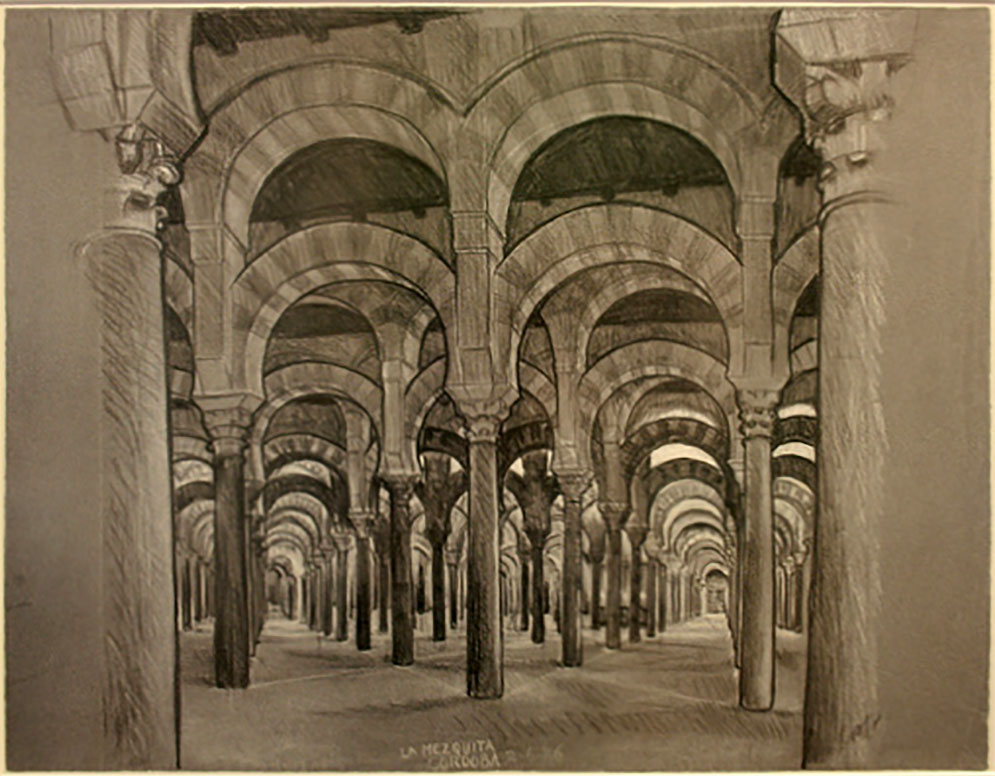
\includegraphics{img_045.jpg}
\caption[清真寺,艾舍尔作。]
  {清真寺,艾舍尔作(黑白粉笔画,1936)。}
\end{figure}

\item[乌龟]嗯……听来好像你所做的只是把对一个判定过程的需求转换到了另一个领域。现在你所需要的是一个判定佛性的过程。下一个呢?说到底,要是你甚至不能说出一只狗是否有佛性,你又怎么能判定每个可能的折叠串是否有佛性呢?

\item[阿基里斯]呃,我师傅跟我解释说,这种领域转换是有用的。它有些像视点的转换。有时某些事情从一种角度看很复杂,而从另一个角度看却很简单。他以果园为例:从一个角度看,你看不出什么秩序,可是从某些特定的角度,你会发现优美的规律性。通过变换你的观察方式,你就把同一信息重新编排了。

\item[乌龟]我明白了。这么说也许一个公案的正宗性是深藏不露的,而一旦你把它翻译成一个串,它就会以某种方式浮到表层来,是吗?

\item[阿基里斯]这就是我师傅的发现。

\item[乌龟]那我倒很愿意学学这种技巧。不过请先告诉我:你如何把一个公案(一种词语序列)变成一个折起的串(一种三维的东西)呢?它们的性质可完全不同呀。

\item[阿基里斯]这是禅宗里我所了解到的最神秘的事。它分为两个步骤:“转录”和“翻译”。转录一个公案包括用一种拼音写出该公案,这种拼音只包含四种几何符号。该公案的这种拼音翻译形式被称为信使。

\item[乌龟]那些几何符号是什么样儿的?

\item[阿基里斯]它们是由一些六角形和五角形组成的。就像这样\dlnote{(拿起手边的一块餐巾,给乌龟画出下面四种图形)}:
    \begin{center}
    \begin{tikzpicture}[node distance=5mm,
      every node/.style={inner sep=0, minimum size=12mm, regular polygon}]
    \node[draw, regular polygon sides=6]   (A) {};
    \node[draw, regular polygon sides=6,
      shape border rotate=30, right= of A] (B) {};
    \node[regular polygon sides=6,
      shape border rotate=30, right= of B] (C) {};
    \node[shift=(C.east), xshift=3mm, minimum size=10mm,
      regular polygon sides=5,
      shape border rotate=54, anchor=west] (D) {};
    \node[minimum size=10mm,
      regular polygon sides=5,
      shape border rotate=18, right= of D] (E) {};
    \node[shift=(E.east), xshift=3mm,
      regular polygon sides=6,
      shape border rotate=30, anchor=west] (F) {};
    \coordinate (O) at ($(C.east)!.5!(D.west)$);
    \coordinate (P) at (O |- D.corner 1);
    \coordinate (Q) at (O |- D.corner 2);
    \draw (P) -- (Q)
          (P) foreach \x in {1,2,3,4} { -- (C.corner \x) } --
          (Q) foreach \x in {3,4,5}   { -- (D.corner \x) } -- cycle;
    \coordinate (O) at ($(E.east)!.5!(F.west)$);
    \coordinate (P) at (O |- F.corner 2);
    \coordinate (Q) at (O |- F.corner 3);
    \draw (P) -- (Q)
          (P) foreach \x in {1,2,3}   { -- (E.corner \x) } --
          (Q) foreach \x in {4,5,6,1} { -- (F.corner \x) } -- cycle;
    \end{tikzpicture}
    \end{center}

\item[乌龟]它们看上去挺神秘的。

\item[阿基里斯]只是对没入道的人才显得神秘。一旦你把信使做好之后,你就用手揉好一块口香核糖,然后——

\item[乌龟]口香核糖?是一种特殊的口香糖吗?

\item[阿基里斯]不完全是,折起的串是靠它来保持其形状的。

\item[乌龟]这种核糖是什么做的?

\item[阿基里斯]不清楚,不过它有点像某种胶质的东西,很好用。不管怎么说,你手里一旦有了口香核糖,就可以把信使里的符号序列翻译成某种折叠好的串,就这么简单。

\item[乌龟]慢点儿,别太快了!这些事你怎么做?

\item[阿基里斯]串最初完全是直的,你先从一头开始,按照信使里的几何符号把它折叠成各种形状。

\item[乌龟]每一种几何符号都代表了各不相同的串的折叠方式,是吗?

\item[阿基里斯]不是分别代表。你每次得用三种,而不是一种。你先从串的一头开始,同时也从信使的一头开始。怎样折叠该串的第一寸是由最初三个几何符号决定的。接着的三个符号会告诉你如何折叠串的下一寸。就这样你顺着串同时也顺着信使,一寸寸地把串折叠成一个个小节,直到你用完信使为止。要是你能正确地使用口香核糖,串会保持住它的折叠形状。因此,最后结果是你把该公案翻译成为一个串。

\item[乌龟]过程倒挺漂亮,你用这种办法肯定会得到些奇妙的串。

\item[阿基里斯]那是当然啦。那些长点的公案会被翻译成各种古里古怪的形状。

\item[乌龟]可以想象。不过,为了把信使翻译成串,你必须知道信使中的每三个几何符号代表哪一类折叠。这你怎么知道呢?你有一本字典吗?

\item[阿基里斯]有——一本列有“几何编码”的伟大的书,要是你没有这么一本书,你当然无法把公案翻译成串。

\item[乌龟]当然没办法。这种几何编码是谁搞出来的?

\item[阿基里斯]是由一位名叫戴懋的古人搞出来的。我的师傅说他是唯一一个达到“元顿悟”的人。

\item[乌龟]鼋顿悟?听起来更像一种我能获得的顿悟。可他是个人啊,怎么能达到乌龟顿悟?

\item[阿基里斯]你听岔了,龟兄,我说的是元顿悟,不是鼋顿悟。你还不可能顿悟呢。要是咱们俩之间非得有一个达到顿悟的话,那也只能是“顿吾”,你甚至连顿悟的第一个阶段还没达到呢,更别说——

\item[乌龟]谁知道,阿基。也许那些了解顿悟三昧的人会返归于顿悟前的状态。我总是认为“顿悟两次即是没顿悟”。不过,还是让我们回到玳瑁——唔,我是说,戴懋上来吧。

\item[阿基里斯]除了知道他还发明了禅宗串技艺外,我们几乎对他一无所知。

\item[乌龟]发明了什么?

\item[阿基里斯]发明了凭借它可以判定佛性的一种技艺。我会跟你讲的。

\item[乌龟]我会着迷的。对我这么个刚入法门的人来说,要知道的东西太多了!

\item[阿基里斯]据说有一个公案专门讲禅宗串技艺是怎么来的。但不幸的是,这一切早已随着时间的流逝而遗失掉了,无疑是永远遗失了。这也倒好,要不然准会有些盗用这位大师之名的模仿者,各行其是地仿造它。

\item[乌龟]可是,如果所有禅众都效仿那个最顿悟的禅师——戴懋,这不是件好事吗?

\item[阿基里斯]我来给你讲一个关于模仿者的公案吧。
\begin{quote}
俱胝和尚,凡有诘问,惟举一指。后有童子,因外人问:“和尚说何法要?”童子亦竖指头。胝闻,遂以刃断其指,童子负痛号哭而去。胝复召之,童子回首,胝却竖起指头,童子忽然领悟。
\end{quote}

\item[乌龟]嘿,太有趣了!刚才我以为禅宗就是赵州和他的那些小把戏,现在我发现倶胝也挺可爱。他看来很有点幽默感。

\item[阿基里斯]这个公案很严肃。我不知道你怎么会觉得它幽默。

\item[乌龟]也许正是因为这种幽默才使得禅宗富于教益。我想如果你十分严肃地看待这些故事,那你既会有所得也会有所失。

\item[阿基里斯]也许对你的这种乌龟禅来说有道理。

\item[乌龟]你能回答我一个问题吗?就一个。我想知道菩提达摩为什么从印度来到中国?

\item[阿基里斯]哦!我可以告诉你赵州被问及这一问题时怎么说的吗?

\item[乌龟]请吧。

\item[阿基里斯]他回答说:“庭前柏树子。”

\item[乌龟]挺合情合理,我也会这么说。只是把它用来回答一个与此不同的问题,也就是说,用来回答:“烈日当空的时候,到哪儿去找个荫凉地儿?”

\item[阿基里斯]你还不知道,你已经无意中触到了禅宗的一个最基本的问题。这个问句听起来平淡无奇,实际上却是在问:“禅宗的基本原理是什么?”

\item[乌龟]太伟大了,我一点也没想到禅宗的核心目的就是要找个荫凉地儿。

\item[阿基里斯]噢,不——你完全误解了我的意思。我指的不是那个问题。我是指你的那个菩提达摩为何从印度来到中国的问题。

\item[乌龟]我明白了。嗯,没想到我已经涉及到这么深的领域了。不过还是让我们回到这个奇特的映射上来吧。我已经了解到任何公案都可以照你讲的方法转换成某种折叠的串。那么,把这个过程倒过来会怎么样?折叠的串能够用这种方法被释读为一个公案吗?

\item[阿基里斯]嗯,在某种意义上可以。不过……

\item[乌龟]怎么啦?

\item[阿基里斯]你最好不要把它倒过来。这会违背禅宗串的中心法则,你瞧,这种法则是这样的\dlnote{(拿起一块餐巾往上画)}:
    \begin{center}
    \begin{tabular}{ccccc}
     公案  & $\Longrightarrow$ & 信使 & $\Longrightarrow$ & 折叠的串 \\
         & 转录                                 &     & 翻译
    \end{tabular}
    \end{center}
你不能逆着箭头的方向做——尤其是第二个箭头。

\item[乌龟]告诉我,法则还有佛性也无?我应该废问这个问题,是吗?

\item[阿基里斯]你废问这个问题,我很高兴。但是——我想向你分享一个秘密。你保证不对任何人讲吗?

\item[乌龟]以龟格担保。

\item[阿基里斯]那好吧。有一次,我真的逆箭头了。我觉得我得出了一种不合教规但却激动人心的结果。

\item[乌龟]嗬,阿基!想不到你居然还会做出这么不虔诚的事来。

\item[阿基里斯]我以前从没有向别人坦白过——甚至包括蟹尊。

\item[乌龟]那么告诉我,你逆着中心法则中的箭头做发生什么事了?是不是说你从一个串开始,最后得出一个公案?

\item[阿基里斯]有时是这样——可是还出现了些更古怪的东西呢。

\item[乌龟]比产生一个公案还古怪吗?

\item[阿基里斯]对……当你倒译和倒录时,你能得出某种东西,不过,并不总是公案。某些串用这种方式大声读出时毫无意义。

\item[乌龟]毫无意义?这不正是公案的别名吗?

\item[阿基里斯]你显然还不具备真正的禅宗精神。

\item[乌龟]至少你总还得到了些故事吧?

\item[阿基里斯]并不总是——有时你得到些毫无意义的音节,又有时你得到些不合语法的句子。不过偶尔也能得到类似公案的东西。

\item[乌龟]只是类似吗?

\item[阿基里斯]嗯,你知道,它也许是冒牌的。

\item[乌龟]哦,那当然。

\item[阿基里斯]我把这些能得出近乎公案的东西的串称作“良构”的串。

\item[乌龟]可你干嘛不告诉我那个使你能区分正宗公案和冒牌公案的判定过程?

\item[阿基里斯]我正要讲呢。对一个公案(或非公案),首先把它翻译成三维的串。剩下的事就只是确定该串是否具有佛性。

\item[乌龟]可是怎么确定呢?

\item[阿基里斯]嗯,我的师傅说戴懋就行,他只要对一个串瞥上一眼,就能确定它是否具有佛性。

\item[乌龟]可是如果你还没有达到元顿悟的境界怎么办呢?没有别的办法来判断一个串是否具有佛性吗?

\item[阿基里斯]有的。这也正是禅宗串技艺的用武之地。用这种技艺可以做出无数个串,所有这些串都具有佛性。

\item[乌龟]很有意思!是不是还有一种与此对应的方法用来做出不具有佛性的串?

\item[阿基里斯]你为什么要做出不具佛性的串呢?

\item[乌龟]哦,我只是觉得它也许有用。

\item[阿基里斯]你这人真怪,想不到,你对不具佛性的东西比对具佛性的东西还感兴趣!

\item[乌龟]我不是还没顿悟嘛!讲下去吧,告诉我怎样做出一个具有佛性的串。

\item[阿基里斯]嗯,开始时,你得先把一个串挂在你的双手上,让它处于五种合法的初始形状中的一种,就像这样……\dlnote{(拿起一个串,把它弄成圈状,挂在每只手伸出的一个个指头之间)}。

\item[乌龟]另外那四种合法的初始形状是什么样的?

\item[阿基里斯]每种位置都被看做是一种挂住一个串的自明的方法,甚至连新手都能以那些姿式挂起串。而这五个串都具有佛性。

\item[乌龟]当然。

\item[阿基里斯]另外还有一些串处理规则,凭着它们你可以做出更复杂的串图形,特别是,你可以通过双手的一些基本动作来调整串。比方说,你可以这样叉起手指——也可以这样伸开——还可以这样绞起。每一次操作都会使挂在你双手上的串彻底改变形状。

\item[乌龟]嘿,摆弄这些串的办法看上去就像玩挑绷子游戏一样!

\item[阿基里斯]没错儿。你现在好好看着它们,这些规则中有一些可以使串更复杂,有一些会把它们简化,但是不管你想得到哪种结果,只要你遵守串的处理规则,你做出的每个串就都具有佛性。

\item[乌龟]真是妙极了。那么,隐藏在你刚做成的那个串中的公案怎么样啦?它是正宗的吗?

\item[阿基里斯]嗯,据我所知,它一定是正宗的。因为我是依照规则,先从五种自明的形状中的一种开始做的,所以这个串一定具有佛性,因而它必然对应于一个正宗的公案。

\item[乌龟]你知道这个公案是什么吗?

\item[阿基里斯]你想引我违反中心法则吗?嘿。你这坏家伙!

\dnote{(阿基里斯皱着眉头,手里拿着编码字典,沿着那个串一寸一寸划划点点,记录着代表公案的由三个几何符号构成的奇特拼音,直到差不多记满了一块餐巾。)}

好啦!

\item[乌龟]真了不起。让我们听听它怎么说吧。

\item[阿基里斯]行啊。

  \begin{quote}
  赵州因僧问婆子:“台山路向甚处去?”

  婆云:“蓦直去。”

  僧才行三五步,婆云:“好个师僧又恁麽去!”

  后有僧举似赵州,州云:“待我去与你勘过这婆子。”

  明日便去,亦如是问,婆亦如是答。

  州归谓众曰:“台山婆子,我与你勘破了也。”
 \end{quote}

\item[乌龟]嗬,他简直跟福尔摩斯一样神,联邦调查局没雇赵州真是太可惜了。告诉我——要是我也遵守禅宗串技艺中的规则,我也能做出来,对吗?

\item[阿基里斯]对。

\item[乌龟]我应该按照你的操作顺序做吗?

\item[阿基里斯]不必,任何顺序都可以。

\item[乌龟]当然啦,那样一来我就会得出一个与此不同的串,因而也会得到一个不同的公案。我是不是得按照与你一样多的步骤做呢?

\item[阿基里斯]用不着。多少步都可以。

\item[乌龟]好吧,那么就会有无数的具有佛性的串——因此也会有无数正宗公案了!你怎么能知道有些串不能由你的规则做出呢?

\item[阿基里斯]哦,对啦——让我们回到缺乏佛性的事情上来吧。是这样的:你一旦知道了如何做出具有佛性的串,你也就能够做出不具有佛性的串。这是我师傅从一开始就诲谕我的。

\item[乌龟]妙极了!怎么个做法呢?

\item[阿基里斯]很容易,先举做缺乏佛性的串的例子……

\dnote{(他拿起那个从中“拉出了”前面那个公案的串,在它的一头儿打了个弯,其状如“~”。)}

这就是个无佛性的。

\item[乌龟]很清楚。要做的只是再加上一个“弯”,是吗?你怎么知道这个新串缺乏佛性?

\item[阿基里斯]这是因为佛性的基本性质:当两个良构串除了其中一个的一端有一个“弯”以外完全相同时,两者中只有一个具有佛性。这只是我师傅观察到的经验。

\item[乌龟]我在考虑一件事:是否存在某些不管你以哪种顺序按照禅宗串规则都无法得到的具有佛性的串?

\item[阿基里斯]我真不愿承认,在这一点上我自己也有点糊涂。起初,我师傅强调说,一个串中的佛性是先由五个合法的初始形状之中的某一个、然后按照允许使用的规则来展开这样一个过程所规定的。可是后来,他说起什么人的“定理”。我一直没弄懂,说不定我甚至听差了,但是不管他说了什么,总之使我怀疑用这种方法是否能囊括全部有佛性的串。据我所知,这种事是有的。不过,佛性是种很难理解的东西。

\item[乌龟]从赵州的“无”那里我已经猜到一些了。我想……

\item[阿基里斯]想什么?

\item[乌龟]我是在想那两个公案——我是说那个公案和它的反公案——一个说“即心是佛”,另一个说“即心非佛”——用几何编码把它们转化成串后,会是什么样呢?

\item[阿基里斯]我很愿意让你看看。

\dnote{(他写下拼音转录式,然后从他的串袋里拿出一对串,把每个串上的每一段都按那个奇特的符号表中的一个三元组折叠起来。最后,他把弄好的串并排摆好。)}

你瞧,这就是不同之处。

\item[乌龟]它们确实非常相像。我相信它们之间只有一处不同:这一个的一端上有一个“弯”!

\item[阿基里斯]向赵州保证,你说对了。

\item[乌龟]哈!现在我明白你师傅为什么怀疑了。

\item[阿基里斯]你明白了?

\item[乌龟]根据你的那个经验之谈,这一对中至多有一个具有佛性,因此你也就知道公案中有一个必定是冒牌的。

\item[阿基里斯]但是这并没有说出哪一个是冒牌的。我试过,我师傅也试过,用串处理规则来做出两个串,可是行不通,一个也没有做出来,真叫人沮丧,有时你甚至会怀疑……

\item[乌龟]你是说,会怀疑两者中是否必有一个具有佛性?说不定两个都不具有佛性——两个公案都不是正宗的!

\item[阿基里斯]我从来没有想那么远——不过你是对的——我想这是可能的。但我想你不应该就佛性问这么多的问题。无门禅师总是警告他的弟子过多地提问题是危险的。

\item[乌龟]好吧——不再问了。不过我很想自己作出一个串。看看我做出来的是否是良构串,这会是非常有趣的。

\item[阿基里斯]会很有趣的。这是一个串。\dlnote{(他递给乌龟一个串。)}

\item[乌龟]你看,我一点也不知道该怎么去做。对我这个蹩脚产品,就请你多包涵了。它不会遵循任何规则,而且可能会搅缠在一起无法释读。\dlnote{(他抓住双脚间的圈,作了一些简单处理,得到了一个复杂的串,默默地递给阿基里斯。这时,阿基里斯兴奋起来。)}

\item[阿基里斯]咦唏!我得用你的这种方法试试。我从未见过这样的串!

\item[乌龟]我希望它是良构的。

\item[阿基里斯]我看到它的一头有个“弯”。

\item[乌龟]噢——等等!我先拿回来一下可以吗?我想再鼓捣一下。

\item[阿基里斯]啊,当然可以。给。

\dnote{(把它交还给乌龟,乌龟在同一头又打了个“~”,然后猛地一拉,两个“~”顿时都没了!)}

\item[阿基里斯]怎么回事?

\item[乌龟]我想去掉那个“弯”。

\item[阿基里斯]可是,你并没有去弄直它,而是又打了一个,然后两个都没了!它们到哪儿去了?

\item[乌龟]当然是跑到堕界去了。这就是双重打“弯”律。

\dnote{(突然,两个“~”不知从哪儿冒了出来——也就是说,从堕界里冒了出来。)}

\item[阿基里斯]有意思。如果它们能这么轻易地从堕界中跳出跳进,那它们一定是待在堕界的一个出入方便的层里。不然就是堕界的所有地方出入难度都相同?

\item[乌龟]我说不上。不过,在我看来,如果烧掉这个串就会使这两个“弯”不能重现。在这种情况下,你应该认为它们是呆在堕界的深层里。说不定堕界有好多好多层呢。不过这无所谓。我想要知道的只是,如果你把我的串转换成拼音符号,它们会怎么样。\dlnote{(当他把它递过去的时候,两个小“~”又一次不见了。)}

\item[阿基里斯]我总是为违反中心法则而深感内疚……

\dnote{(拿出笔和编码字典,仔细而匆忙地用许多三个一组的符号记下对应的缠绕在一起的乌龟的串,记完以后,他清了清嗓子。)}

啊哼。你想听听你做出的东西吗?

\item[乌龟]如果你愿意,我当然愿意。

\item[阿基里斯]好吧。是这样的:
  \begin{quote}
  玳瑁屡因僧问:“物皆具佛性也无?”\lnote{(盖玳瑁乃唯一获元顿悟者。)}恒趺坐不语。凡僧所问及者,已涉豆菽、湖沼、月夜等。一日,僧示之以一串,问该串亦具佛性也无。竟默然劈手攫过其串挂于双足间,且——
  \end{quote}

\item[乌龟]在他的双足之间?真奇了!

\item[阿基里斯]你怎么会觉得它真奇了呢?

\item[乌龟]嗯,啊……你有点道理。但是接着讲吧!

\item[阿基里斯]好吧。
  \begin{quote}
  竟默然劈手攫过其串挂于双足间,且稍事作弄,竟成一串,叠套纠缠,繁复非常。乃默然与僧,僧便豁然顿悟。
  \end{quote}

\item[乌龟]要是我,我宁愿双重顿悟。

\item[阿基里斯]只要你从挂在你双脚间的串开始,那它就会告诉你怎样做出玳瑁的串。让我跳过那些讨厌的细节吧。它的结尾是:
  \begin{quote}
  僧自此不复诘问。而仿玳瑁之技造串不已,传造串之技于其弟子,其弟子复以教它人焉。
  \end{quote}

\item[乌龟]真是奇文。真不敢相信它就藏在我的串里。

\item[阿基里斯]可它就藏在里面。更令人吃惊的是,你似乎一下子就做出了一个良构串。

\item[乌龟]可是,玳瑁的串是什么样的?我想这是这个公案的关键所在。

\item[阿基里斯]我怀疑这一点。人们不应该“执于”公案内部的细节。重要的是整个公案的精神,不是它的一部分。哦,这太有意思了!我想——虽然听起来很不合情理——你可能已经找到了那个遗失了很久的、用来描述禅宗串技艺起源的公案了!

\item[乌龟]嗬,那太好了,简直好得不能具有佛性了。

\item[阿基里斯]可是,这就说那位禅师——那个唯一达到过元顿悟的神秘状态的人——的名字叫“玳瑁”,而不是“戴懋”。多滑稽的名字!

\item[乌龟]我不同意。我觉这个名字挺漂亮的。我还想知道玳瑁的串是什么样儿。你能根据那个公案中的描述把它重做出来吗?

\item[阿基里斯]我可以试试……当然,我也得用我的双脚,因为它是用脚的动作描述的。这很不寻常。不过我想我能对付。我来试试。

\dnote{(他拿起那个公案和一个串,把那个串又拧又弯,不消几分钟,他就用这种神祕方法得出一个东西来。)}

好了,瞧。怪哉,它看起来好眼熟啊。

\item[乌龟]啊,可不是吗!我在哪儿见过它,只是想不起来了。

\item[阿基里斯]我知道了!嘿。这是你的串,龟兄!是不是?

\item[乌龟]确实不是。

\item[阿基里斯]确实不是——它正是你第一次递给我时的那个串,你给我的那个时候它上边还没有第二个“弯”呢。

\item[乌龟]哦,对——就是它。真想不到。我不知道这里有什么含义。

\item[阿基里斯]至少是挺怪的。

\item[乌龟]你认为我的公案是正宗的吗?

\item[阿基里斯]请等一会儿……

\item[乌龟]我的串具有佛性吗?

\item[阿基里斯]龟兄,你的串开始叫我感到不安了。

\item[乌龟]\dlnote{(一副很得意的样子,一点也没有注意阿基里斯)}玳瑁的串怎么样?它具有佛性吗?我有一堆问题要问呢!

\item[阿基里斯]我害怕这些问题了,龟兄。这里出现了些极怪的东西,我不敢说我喜欢它。

\item[乌龟]很抱歉,我无法想象是什么叫你不安。

\item[阿基里斯]嗯,我所知道的解释它的最好方法是援引另一个老禅师香严的话:
  \begin{quote}
  香严和尚云:“\lnote{(禅)}如人上树,口衔树枝,手不攀枝,脚不蹋枝,树下有人问\lnote{(如何是祖师)}西来意?不对,即违他问;若对,又丧身失命。正恁麼时,作麼生对?”
  \end{quote}

\item[乌龟]很清楚:他就应该放弃禅宗,改学分子生物学。

\end{dialogue}

\end{dialog}
